% !TEX encoding = UTF-8
% !TEX program = pdflatex
% !TEX options = -synctex=1 -interaction=nonstopmode -file-line-error -recorder "%DOC%"

\documentclass{beamer}

\usepackage{listings}
\usepackage{url}
\usepackage{xcolor}
\usepackage{sourcecodepro}
\usepackage{tikz}
\usepackage{tikz-qtree}

% There are many different themes available for Beamer. A comprehensive
% list with examples is given here:
% http://deic.uab.es/~iblanes/beamer_gallery/index_by_theme.html
% You can uncomment the themes below if you would like to use a different
% one:
%\usetheme{AnnArbor}
%\usetheme{Antibes}
%\usetheme{Bergen}
%\usetheme{Berkeley}
%\usetheme{Berlin}
%\usetheme{Boadilla}
%\usetheme{boxes}
%\usetheme{CambridgeUS}
%\usetheme{Copenhagen}
%\usetheme{Darmstadt}
%\usetheme{default}
%\usetheme{Frankfurt}
%\usetheme{Goettingen}
%\usetheme{Hannover}
%\usetheme{Ilmenau}
%\usetheme{JuanLesPins}
%\usetheme{Luebeck}
\usetheme{Madrid}
%\usetheme{Malmoe}
%\usetheme{Marburg}
%\usetheme{Montpellier}
%\usetheme{PaloAlto}
%\usetheme{Pittsburgh}
%\usetheme{Rochester}
%\usetheme{Singapore}
%\usetheme{Szeged}
%\usetheme{Warsaw}

\lstset{
    columns=fixed,
    numbers=left,
    basicstyle=\ttfamily\scriptsize,
    breaklines=true,
    keywordstyle=\color[RGB]{40, 40, 255},
    numberstyle=\scriptsize\color{darkgray},
    commentstyle=\ttfamily\color[RGB]{0, 128, 96},
    stringstyle=\ttfamily\color[RGB]{192, 0, 0},
    showstringspaces=false,
    morekeywords={alignas,continute,friend,register,true,alignof,decltype,goto,
    reinterpret_cast,try,asm,defult,if,return,typedef,auto,delete,inline,short,
    typeid,bool,do,int,signed,typename,break,double,long,sizeof,union,case,
    dynamic_cast,mutable,static,unsigned,catch,else,namespace,static_assert,using,
    char,enum,new,static_cast,virtual,char16_t,char32_t,explict,noexcept,struct,
    void,export,nullptr,switch,volatile,class,extern,operator,template,wchar_t,
    const,false,private,this,while,constexpr,float,protected,thread_local,
    const_cast,for,public,throw,std,uint16,uint16_t,uint32,uint32_t,table,union},
}

\newcommand{\cpp}{C\texttt{++}}

\title{An online drawboard}
\subtitle{Final project for Exercise on Operating Systems}

\author{zheng qian (xqq)}
% - Give the names in the same order as the appear in the paper.
% - Use the \inst{?} command only if the authors have different
%   affiliation.

\institute[SIT] % (optional, but mostly needed)
{
  Department of Computer Science and Engineering\\
  Shibaura Institute of Technology
}

\date{2020/01/20}

\subject{Online drawboard (final project for Exercise on Operating Systems)}
% This is only inserted into the PDF information catalog.

\begin{document}

\begin{frame}
  \titlepage
\end{frame}

\begin{frame}{Open Source}
\begin{center}
Source code has been public released on GitHub
\end{center}
\begin{center}
\url{https://github.com/xqq/drawboard}
\end{center}
\end{frame}

\begin{frame}{Overview}
  \tableofcontents
\end{frame}

% Section and subsections will appear in the presentation overview
% and table of contents.
\section{Motivation}

\begin{frame}{Motivation}{Why try to make an online drawboard}

In the 110 center of Tokyo Metropolitan Police Department,
all of the telephone operator has a drawing board in front of them,
that can sync drawings at realtime with other police officers.

The telephone operator records important information by writing on the drawing board when talking to the reporter.

At the same time, another officer who is responsible for that case,
can look at his drawboard that is realtime-synced with the telephone operator's drawboard.

\end{frame}

\section{Design purpose}

\begin{frame}{Design purpose}
  \begin{itemize}
  \item {
    To be cross-platform but without extra performance degrade

    - We can support Windows, Linux and macOS
  }
  \item {
    Use cross-platform GUI libraries

    - SDL2 for window creating and graphics rendering
  }
  \item {
    To be high performance

    - We can choose high performance languages like C/\cpp

    - Take advantage of multi-threading
  }
  \item {
    Make the code well-orginized

    - Use Modern \cpp  (\cpp 11 / \cpp 14)
  }
  \item {
    There're differences between different platforms's socket API

    - Make seperate implementation for Windows (WinSock) and POSIX

    - and unify to consistent interfaces
  }
  \end{itemize}
\end{frame}


\section{Architecture}

\begin{frame}[fragile]{Architecture}
\begin{columns}[c] % The "c" option specifies centered vertical alignment while the "t" option is used for top vertical alignment

\column{.5\textwidth} % Left column and width
\begin{lstlisting}[language=c++,numbers=none,basicstyle=\ttfamily\tiny]
|-- client
|   -- client_app.cpp
|   -- client_app.hpp
|   -- draw_client.cpp
|   -- draw_client.hpp
|   -- sdl_include.hpp
|-- common
|   -- abstract_canvas.cpp
|   -- abstract_canvas.hpp
|   -- blocking_queue.hpp
|   -- log.cpp
|   -- log.hpp
|   -- noncopyable.hpp
|   -- packet.cpp
|   -- packet.hpp
|   -- threaded_worker.cpp
|   -- threaded_worker.hpp
|-- protocol
|   -- protocol.fbs
|   -- protocol_generated.h
\end{lstlisting}

\column{.45\textwidth} % Right column and width
\begin{lstlisting}[language=c++,numbers=none,basicstyle=\ttfamily\tiny]
|-- server
|   -- draw_server.cpp
|   -- draw_server.hpp
|   -- task.hpp
|   -- transmit_worker.cpp
|   -- transmit_worker.hpp
|-- socket
|   -- read_write_buffer.cpp
|   -- read_write_buffer.hpp
|   -- tcp_listener.cpp
|   -- tcp_listener.hpp
|   -- tcp_listener_posix.cpp
|   -- tcp_listener_posix.hpp
|   -- tcp_listener_winsock.cpp
|   -- tcp_listener_winsock.hpp
|   -- tcp_socket.cpp
|   -- tcp_socket.hpp
|   -- tcp_socket_posix.cpp
|   -- tcp_socket_posix.hpp
|   -- tcp_socket_winsock.cpp
|   -- tcp_socket_winsock.hpp
|-- thirdparty
|   |-- argh/
|   |-- flatbuffers/
|-- main.cpp
|-- CMakeLists.txt
\end{lstlisting}

\end{columns}
\end{frame}


\section{Protocol}

\begin{frame}[fragile]{Protocol}{Packet \& PacketHeader}
\begin{lstlisting}[language=c++]
struct Packet {
    PacketHeader header;
    PacketPayload payload;
};


struct PacketHeader {
    uint16_t packet_type;
    uint16_t payload_length;
};
\end{lstlisting}

We can determine the packet type \& packet size by parsing packet header
\end{frame}

\begin{frame}[fragile]{Protocol}{PacketPayload (flatbuffers)}
\begin{lstlisting}[language=c++]
table PacketPayload {
    payload: Payload;
}

union Payload {
    ServerHelloPayload,
    FullImagePayload,
    StartDrawPayload,
    EndDrawPayload,
    DrawPointsPayload,
    DeleteBatchPayload,
    UserEnterPayload,
    UserLeavePayload
}
\end{lstlisting}

\begin{itemize}
    \item {
        These structures are defined in google's flatbuffers format.
    }
\end{itemize}
\end{frame}

\begin{frame}[fragile]{Protocol}{StartDrawPayload (flatbuffers)}
\begin{lstlisting}{language=c++}
    table StartDrawPayload {
        uid: uint32;
        sequence_id: uint32;
        color: uint32;
    }
\end{lstlisting}

\begin{itemize}
    \item {
        If user press down left mouse button, client will send such a packet to server
    }
    \item {
        Each user joined the server has an unique uid (UserID)
    }
    \item {
        sequence\_id marks the unique id of drawing operation
    }
    \item {
        color field records the pencil color in ARGB (uint32)
    }
\end{itemize}
\end{frame}

\begin{frame}[fragile]{Protocol}{DrawPointsPayload (flatbuffers)}
\begin{lstlisting}{language=c++}
    struct Vec2 {
        x: int16;
        y: int16;
    }

    table DrawPointsPayload {
        uid: uint32;
        sequence_id: uint32;
        points: [Vec2];
    }
\end{lstlisting}

\begin{itemize}
    \item {
        When user's mouse has moved, client sends mouse coordinates to server
    }
    \item {
        points array stores the mouse coordinates during mouse moving
    }
\end{itemize}
\end{frame}

\begin{frame}[fragile]{Protocol}{DeleteBatchPayload (flatbuffers)}
\begin{lstlisting}{language=c++}
    table DeleteBatchPayload {
        uid: uint32;
        sequence_id: uint32;
    }
\end{lstlisting}

\begin{itemize}
    \item {
        When user pressed Ctrl+Z for Undo, client sends DeleteBatch packet to server
    }
    \item {
        etc... (other payload types are omitted here)
    }
\end{itemize}
\end{frame}

\begin{frame}[fragile]{Protocol: How to parse received data}
{TCP is actually a stream, not separated data packets}
\begin{lstlisting}[language=c++,basicstyle=\ttfamily\tiny]
void ParseBuffer(ReadWriteBuffer* buffer, PacketCallback callback) {
    size_t readable = buffer->GetReadableLength();

    while (readable > sizeof(PacketHeader)) {
        Packet packet;
        // We have to know the size of the new packet, by reading and parsing the header
        buffer->Read(reinterpret_cast<uint8_t*>(&packet.header), sizeof(packet.header));

        readable = buffer->GetReadableLength();
        // If remained data could not make up an complete payload, rollback and wait for next
        if (readable < packet.header.payload_length()) {
            buffer->RollbackReadPointer(sizeof(packet.header));
            break;
        }

        size_t payload_length = packet.header.payload_length();

        packet.payload_buffer.resize(payload_length);
        buffer->Read(packet.payload_buffer.data(), payload_length);
        readable = buffer->GetReadableLength();

        packet.payload = GetPacketPayload(packet.payload_buffer.data());
        callback(std::move(packet));
    }
}
\end{lstlisting}

\end{frame}


\section{Socket}

\begin{frame}[fragile]{TcpSocket}
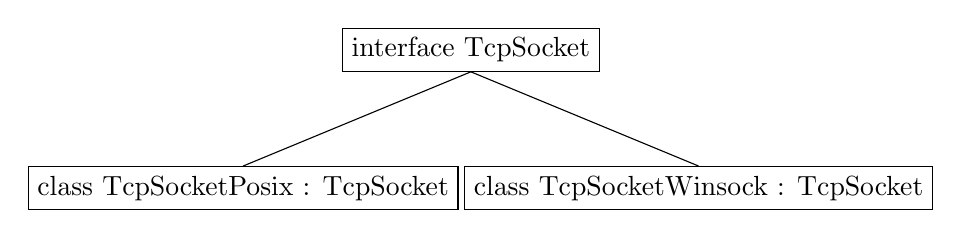
\begin{tikzpicture}
    \tikzset{level distance=50pt}
    \Tree [.\node[draw]{interface TcpSocket};
        [.\node[draw]{class TcpSocketPosix : TcpSocket}; ]
        [.\node[draw]{class TcpSocketWinsock : TcpSocket}; ]
    ]
\end{tikzpicture}
\newline
\begin{lstlisting}[language=c++]
class TcpSocket {
public:
    TcpSocket() {}
    virtual ~TcpSocket() {}
    virtual void SetCallback(OnConnectedCallback on_connect,
                             OnDisconnectCallback on_disconnect,
                             OnDataArrivalCallback on_arrival,
                             OnErrorCallback on_error) = 0;
    virtual bool Connect(std::string connect_addr, uint16_t port) = 0;
    virtual bool Send(const uint8_t* buffer, size_t length) = 0;
    virtual bool Shutdown() = 0;
}
\end{lstlisting}
\end{frame}

\begin{frame}[fragile]{TcpListener}
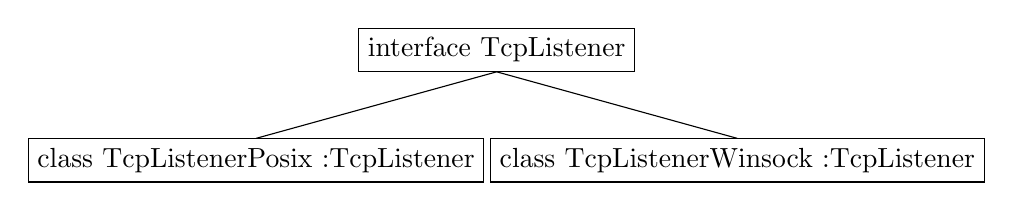
\begin{tikzpicture}
    \tikzset{level distance=40pt}
    \Tree [.\node[draw]{interface TcpListener};
        [.\node[draw]{class TcpListenerPosix :TcpListener}; ]
        [.\node[draw]{class TcpListenerWinsock :TcpListener}; ]
    ]
\end{tikzpicture}
\newline
\begin{lstlisting}[language=c++]
class TcpListener {
public:
    TcpListener(OnAcceptedCallback on_accept, OnErrorCallback on_error);
    virtual ~TcpListener() {}
    virtual bool StartListen(std::string bind_addr, uint16_t port) = 0;
    virtual bool EndListen() = 0;
};
\end{lstlisting}
\end{frame}


\begin{frame}[fragile]{WinSock}
{Windows's WinSock API is a little bit different from POSIX socket}
Before calling any WinSock API, it's necessary to do initialize
\begin{lstlisting}[language=c++,basicstyle=\ttfamily\tiny]
WSADATA wsa_data;
int ret = WSAStartup(MAKEWORD(2, 2), &wsa_data);
if (ret != 0) {
    on_error_(this, "WSAStartup failed");
}
\end{lstlisting}
\small{WinSock API is a bit different from POSIX, like using closesocket() rather than close()}
\begin{lstlisting}[language=c++,basicstyle=\ttfamily\tiny]
socket_ = socket(result->ai_family, result->ai_socktype, result->ai_protocol);
if (socket_ == INVALID_SOCKET) {
    on_error_(this, "socket() creation failed");
    freeaddrinfo(result);
    return false;
}

ret = connect(socket_, result->ai_addr, static_cast<int>(result->ai_addrlen));
if (ret == SOCKET_ERROR) {
    on_error_(this, "connect() failed");
    closesocket(socket_);
    socket_ = 0;
    freeaddrinfo(result);
    return false;
}

freeaddrinfo(result);
\end{lstlisting}
\end{frame}


\section{Multi-threading architecture}

\begin{frame}[fragile]{TcpSocket threading}
Each TcpSocket will create a separate thread for recv()
\begin{lstlisting}[language=c++,basicstyle=\ttfamily\tiny]
void TcpSocketPosix::ThreadWorker() {
    ReadWriteBuffer buffer(4096);
    uint8_t buf[512] = {0};

    while (true) {
        ssize_t nread = recv(fd_, buf, sizeof(buf), 0);

        if (nread == 0) {
            // connection closing
            close(fd_);
            fd_ = 0;
            on_disconnect_(this);
            break;
        } else if (nread == -1) {
            close(fd_);
            fd_ = 0;
            on_error_(this, "recv() returned with error");
            break;
        }

        buffer.Write(buf, static_cast<size_t>(nread));
        on_arrival_(this, &buffer, (size_t)nread);
        memset(buf, 0, sizeof(buf));
    }
}
\end{lstlisting}
\end{frame}

\begin{frame}[fragile]{TcpSocket threading}{Create new thread after connect() complete}
\begin{lstlisting}[language=c++,basicstyle=\ttfamily\tiny]
bool TcpSocketPosix::Connect(std::string connect_addr, uint16_t port) {
    assert(fd_ == 0);
    fd_ = socket(AF_INET, SOCK_STREAM, 0);

    int enable = 1;
    if (setsockopt(fd_, IPPROTO_TCP, TCP_NODELAY, &enable, sizeof(enable)) == -1) {
        on_error_(this, "setsockopt(TCP_NODELAY) failed");
        return false;
    }

    remote_addr_.sin_family = AF_INET;
    remote_addr_.sin_port = htons(port);
    inet_pton(AF_INET, connect_addr.c_str(), &remote_addr_.sin_addr);

    int ret = connect(fd_, reinterpret_cast<struct sockaddr*>(&remote_addr_), sizeof(remote_addr_));
    if (ret == -1) {
        on_error_(this, "connect() failed");
        return false;
    }

    on_connect_(this);
    // Create worker thread for recv() incoming data
    thread_ = std::thread(&TcpSocketPosix::ThreadWorker, this);
    return true;
}
\end{lstlisting}
\end{frame}

\begin{frame}[fragile]{Server side multi-threading}{Use standalone worker thread for data sending}
All packets to be sent to clients will be pushed into a BlockingQueue
\newline
\begin{lstlisting}[language=c++,basicstyle=\ttfamily\tiny]
void DrawServer::BroadcastPacket(PacketHeader* header, const uint8_t* payload, size_t payload_length) {
    std::vector<uint8_t> packet_buffer(sizeof(*header) + payload_length);

    size_t header_size = sizeof(*header);
    memcpy(packet_buffer.data(), header, header_size);
    memcpy(packet_buffer.data() + header_size, payload, payload_length);

    Task t(TaskType::kBroadcastSend, std::move(packet_buffer));
    task_queue_.Enqueue(std::move(t));
}
\end{lstlisting}
\end{frame}


\begin{frame}[fragile]{Server side multi-threading}{Use standalone worker thread for data sending}
The worker thread always waits on BlockingQueue for a new task,
then dequeue packets from BlockingQueue and send them through sockets
\begin{lstlisting}[language=c++,basicstyle=\ttfamily\tiny]
void TransmitWorker::Run() {
    while (true) {
        task_queue_->Poll();
        if (task_queue_->IsExit()) { // immediate-exit flag
            return;
        }
        Task msg = task_queue_->Dequeue();

        if (msg == TaskType::kPrivateSend) {
            msg.socket->Send(msg.buffer.data(), msg.buffer.size());
        } else if (msg == TaskType::kBroadcastSend) {
            for (auto& iter : *socket_cluster_) {
                TcpSocket* socket = iter.second.get();
                socket->Send(msg.buffer.data(), msg.buffer.size());
            }
        }
    }
}
\end{lstlisting}
Async operation can avoid long-time blocking during onDataArrival callback
\end{frame}


% Placing a * after \section means it will not show in the
% outline or table of contents.
\section*{Summary}

\begin{frame}{Tips}
  \begin{itemize}
  \item
    \alert{CMake} is a better and easier build script rather than GNU makefile
  \item
    \alert{Modern \cpp} is powerful and can make your code more robust
  \item
    Make good use of \alert{open source libraries}
    \begin{itemize}
      \item This project uses SDL2, google flatbuffers, argh
    \end{itemize}
  \item
    Google / Chromium Code Style is worth learning and practice
  \end{itemize}

  \begin{itemize}
  \item
    It's better to use existing networking framework and libraries...
    \begin{itemize}
    \item
      boost::asio (\cpp)
    \item
      libev (C)
    \item
      libuv (C, with Windows IOCP support), is the core of NodeJS
    \item
      etc
  \end{itemize}
  \item
    These presentation slides is written in \alert{\LaTeX}
\end{itemize}
\end{frame}


\begin{frame}
\Huge{\centerline{The End}}
\Huge{\centerline{ }}
\large{\centerline{Thank you}}
\end{frame}

\end{document}
